\begin{frame}
\frametitle{CNN: VGG-16 as example}
\framesubtitle{Input} 

\begin{textblock}{15}(7.67,-0.62)
	\begin{figure}[H]
		\includegraphics[width=0.1\textwidth]{Images/Team/DamienTOOMEY.png} 
	\end{figure}
\end{textblock}

\begin{adjustwidth}{-1.5em}{-1.5em}
\setlength\arraycolsep{2pt}

\[ \overbrace{\begin{array}{ccc}
\begin{pmatrix}
R_{1,1} & R_{1,2} & R_{1,3} & R_{1,4} \\
R_{2,1} & R_{2,2} & R_{2,3} & R_{2,4} \\
R_{3,1} & R_{3,2} & R_{3,3} & R_{3,4} \\
R_{4,1} & R_{4,2} & R_{4,3} & R_{4,4} \\
\end{pmatrix}
& \begin{pmatrix}
G_{1,1} & G_{1,2} & G_{1,3} & G_{1,4} \\
G_{2,1} & G_{2,2} & G_{2,3} & G_{2,4} \\
G_{3,1} & G_{3,2} & G_{3,3} & G_{3,4} \\
G_{4,1} & G_{4,2} & G_{4,3} & G_{4,4} \\
\end{pmatrix}
& \begin{pmatrix}
B_{1,1} & B_{1,2} & B_{1,3} & B_{1,4} \\
B_{2,1} & B_{2,2} & B_{2,3} & B_{2,4} \\
B_{3,1} & B_{3,2} & B_{3,3} & B_{3,4} \\
B_{4,1} & B_{4,2} & B_{4,3} & B_{4,4} \\
\end{pmatrix} \\
& \textcolor{white}{phantom} & \\
\mathcal{I}_{\textcolor{red}{red}} & \mathcal{I}_{\textcolor{green}{green}} & \mathcal{I}_{\textcolor{blue}{blue}} \\
\end{array}}^{\mathcal{I} = \begin{pmatrix}
I_{1,1} & I_{1,2} & I_{1,3} & I_{1,4} \\
I_{2,1} & I_{2,2} & I_{2,3} & I_{2,4} \\
I_{3,1} & I_{3,2} & I_{3,3} & I_{3,4} \\
I_{4,1} & I_{4,2} & I_{4,3} & I_{4,4} \\
\end{pmatrix}}
\]

\end{adjustwidth}
\end{frame}


\begin{frame}
\frametitle{CNN: VGG-16 as example}
\framesubtitle{2D Convolution : only \textbf{3x3 kernel}, \textbf{stride 1}, \textbf{zero padding of thickness 1}} 

\begin{textblock}{15}(7.67,-0.62)
	\begin{figure}[H]
		\includegraphics[width=0.1\textwidth]{Images/Team/DamienTOOMEY.png} 
	\end{figure}
\end{textblock}

\begin{adjustwidth}{-1.5em}{-1.5em}
\setlength\arraycolsep{2pt}
{\fontsize{9.5}{10}\selectfont
\[
\begin{array}{ccc}
\mathcal{I}_{\textcolor{red}{red}} & \mathcal{I}_{\textcolor{green}{green}} & \mathcal{I}_{\textcolor{blue}{blue}} \\
& \textcolor{white}{phantom} & \\
\begin{pmatrix}
{\only<1,3>{0}}{\only<2>{\color{red}\textbf{0}}} & {\only<1>{0}}{\only<2,3>{\color{red}\textbf{0}}} & {\only<1>{0}}{\only<2,3>{\color{red}\textbf{0}}} & {\only<1,2>{0}}{\only<3>{\color{red}\textbf{0}}} & 0 & 0 \\
{\only<1,3>{0}}{\only<2>{\color{red}\textbf{0}}} & {\only<1>{R_{1,1}}}{\only<2,3>{\color{red}\textbf{$R_{1,1}$}}} & {\only<1>{R_{1,2}}}{\only<2,3>{\color{red}\textbf{$R_{1,2}$}}} & {\only<1,2>{R_{1,3}}}{\only<3>{\color{red}\textbf{$R_{1,3}$}}} & R_{1,4} & 0 \\
{\only<1,3>{0}}{\only<2>{\color{red}\textbf{0}}} & {\only<1>{R_{2,1}}}{\only<2,3>{\color{red}\textbf{$R_{2,1}$}}} & {\only<1>{R_{2,2}}}{\only<2,3>{\color{red}\textbf{$R_{2,2}$}}} & {\only<1,2>{R_{2,3}}}{\only<3>{\color{red}\textbf{$R_{2,3}$}}} & R_{2,4} & 0 \\
0 & R_{3,1} & R_{3,2} & R_{3,3} & R_{3,4} & 0 \\
0 & R_{4,1} & R_{4,2} & R_{4,3} & R_{4,4} & 0 \\
0 & 0 & 0 & 0 & 0 & 0\\
\end{pmatrix}
& \begin{pmatrix}
{\only<1,3>{0}}{\only<2>{\color{green}\textbf{0}}} & {\only<1>{0}}{\only<2,3>{\color{green}\textbf{0}}} & {\only<1>{0}}{\only<2,3>{\color{green}\textbf{0}}} & {\only<1,2>{0}}{\only<3>{\color{green}\textbf{0}}} & 0 & 0 \\
{\only<1,3>{0}}{\only<2>{\color{green}\textbf{0}}} & {\only<1>{G_{1,1}}}{\only<2,3>{\color{green}\textbf{$G_{1,1}$}}} & {\only<1>{G_{1,2}}}{\only<2,3>{\color{green}\textbf{$G_{1,2}$}}} & {\only<1,2>{G_{1,3}}}{\only<3>{\color{green}\textbf{$G_{1,3}$}}} & G_{1,4} & 0 \\
{\only<1,3>{0}}{\only<2>{\color{green}\textbf{0}}} & {\only<1>{G_{2,1}}}{\only<2,3>{\color{green}\textbf{$G_{2,1}$}}} & {\only<1>{G_{2,2}}}{\only<2,3>{\color{green}\textbf{$G_{2,2}$}}} & {\only<1,2>{G_{2,3}}}{\only<3>{\color{green}\textbf{$G_{2,3}$}}} & G_{2,4} & 0 \\
0 & G_{3,1} & G_{3,2} & G_{3,3} & G_{3,4} & 0 \\
0 & G_{4,1} & G_{4,2} & G_{4,3} & G_{4,4} & 0 \\
0 & 0 & 0 & 0 & 0 & 0 \\
\end{pmatrix}
& \begin{pmatrix}
{\only<1,3>{0}}{\only<2>{\color{blue}\textbf{0}}} & {\only<1>{0}}{\only<2,3>{\color{blue}\textbf{0}}} & {\only<1>{0}}{\only<2,3>{\color{blue}\textbf{0}}} & {\only<1,2>{0}}{\only<3>{\color{blue}\textbf{0}}} & 0 & 0 \\
{\only<1,3>{0}}{\only<2>{\color{blue}\textbf{0}}} & {\only<1>{B_{1,1}}}{\only<2,3>{\color{blue}\textbf{$B_{1,1}$}}} & {\only<1>{B_{1,2}}}{\only<2,3>{\color{blue}\textbf{$B_{1,2}$}}} & {\only<1,2>{B_{1,3}}}{\only<3>{\color{blue}\textbf{$B_{1,3}$}}} & B_{1,4} & 0 \\
{\only<1,3>{0}}{\only<2>{\color{blue}\textbf{0}}} & {\only<1>{B_{2,1}}}{\only<2,3>{\color{blue}\textbf{$B_{2,1}$}}} & {\only<1>{B_{2,2}}}{\only<2,3>{\color{blue}\textbf{$B_{2,2}$}}} & {\only<1,2>{B_{2,3}}}{\only<3>{\color{blue}\textbf{$B_{2,3}$}}} & B_{2,4} & 0 \\
0 & B_{3,1} & B_{3,2} & B_{3,3} & B_{3,4} & 0 \\
0 & B_{4,1} & B_{4,2} & B_{4,3} & B_{4,4} & 0 \\
0 & 0 & 0 & 0 & 0 & 0 \\
\end{pmatrix} \\
& \textcolor{white}{phantom} & \\
Kernel[:,:,0] & Kernel[:,:,1] & Kernel[:,:,2] \\
\begin{bmatrix}
w_1 & w_2 & w_3 \\
w_4 & w_5 & w_6 \\
w_7 & w_8 & w_9
\end{bmatrix}
& \begin{bmatrix}
w_{10} & w_{11} & w_{12} \\
w_{13} & w_{14} & w_{15} \\
w_{16} & w_{17} & w_{18}
\end{bmatrix}
& \begin{bmatrix}
w_{19} & w_{20} & w_{21} \\
w_{22} & w_{23} & w_{24} \\
w_{25} & w_{26} & w_{27}
\end{bmatrix}
\end{array} 
\]
}


{\only<1>{
\vspace{0.2cm}
\begin{center}
Goal : learn the weights in the kernels
\end{center}	
}}

{\only<2,3>{
{\fontsize{10}{0}\selectfont
\begin{align*}
& w = np.hstack((Kernel[:,:,0].flatten(), Kernel[:,:,1].flatten(), Kernel[:,:,2].flatten())) \\
& \\
& x = np.hstack((\textcolor{red}{Window}.flatten(),\textcolor{green}{Window}.flatten(),\textcolor{blue}{Window}.flatten())) \\
& \\
& {\only<2>{FeatureMap[0,0,0] = ReLU(w.dot(x) + bias) = ReLU(w^T x + bias)}}{\only<3>{FeatureMap[1,0,0] = ReLU(w.dot(x) + bias) = ReLU(w^T x + bias)}}
\end{align*}
}
}}
\end{adjustwidth}
\end{frame}

\begin{frame}
\frametitle{CNN: VGG-16 as example}
\framesubtitle{Feature maps \& Max pooling} 

\begin{textblock}{15}(7.67,-0.62)
	\begin{figure}[H]
		\includegraphics[width=0.1\textwidth]{Images/Team/DamienTOOMEY.png} 
	\end{figure}
\end{textblock}

\begin{itemize}
\item[•] as many feature maps as there are kernels
\item[•] each kernel is detecting a particular feature (edges,texture,...)
\item[•] by adding more kernels, the model can learn to detect more complex features
\item[•] max pooling $ \Rightarrow $ shrinking of the feature maps 
\begin{itemize}
\item[-] no learnable parameters
\item[-] 2x2 kernel
\item[-] stride 2
\item[-] no zero padding
\end{itemize}
\end{itemize}

\[
\begin{pmatrix}
\textcolor{red}{1} & \textcolor{red}{1} & \textcolor{green}{2} & \textcolor{green}{4} \\
\textcolor{red}{5} & \textcolor{red}{6} & \textcolor{green}{7} & \textcolor{green}{8} \\
3 & 2 & \textcolor{blue}{1} & \textcolor{blue}{0} \\
1 & 2 & \textcolor{blue}{3} & \textcolor{blue}{4} \\
\end{pmatrix}
\underbrace{\rightarrow}_{\text{max pooling}}
\begin{pmatrix}
\textcolor{red}{6} & \textcolor{green}{8} \\
3 & \textcolor{blue}{4} \\
\end{pmatrix}
\]

\end{frame}

\begin{frame}
\frametitle{CNN: VGG-16 as example}
\framesubtitle{Bias} 

\begin{textblock}{15}(7.67,-0.62)
	\begin{figure}[H]
		\includegraphics[width=0.1\textwidth]{Images/Team/DamienTOOMEY.png} 
	\end{figure}
\end{textblock}

\[ weighted\_sum = \sum_{i=1}^n w_i x_i = w^T x \]

\begin{itemize}
\item[•] biases are learned parameters
\item[•] each neuron has a bias
\end{itemize}

\begin{figure}[H]
	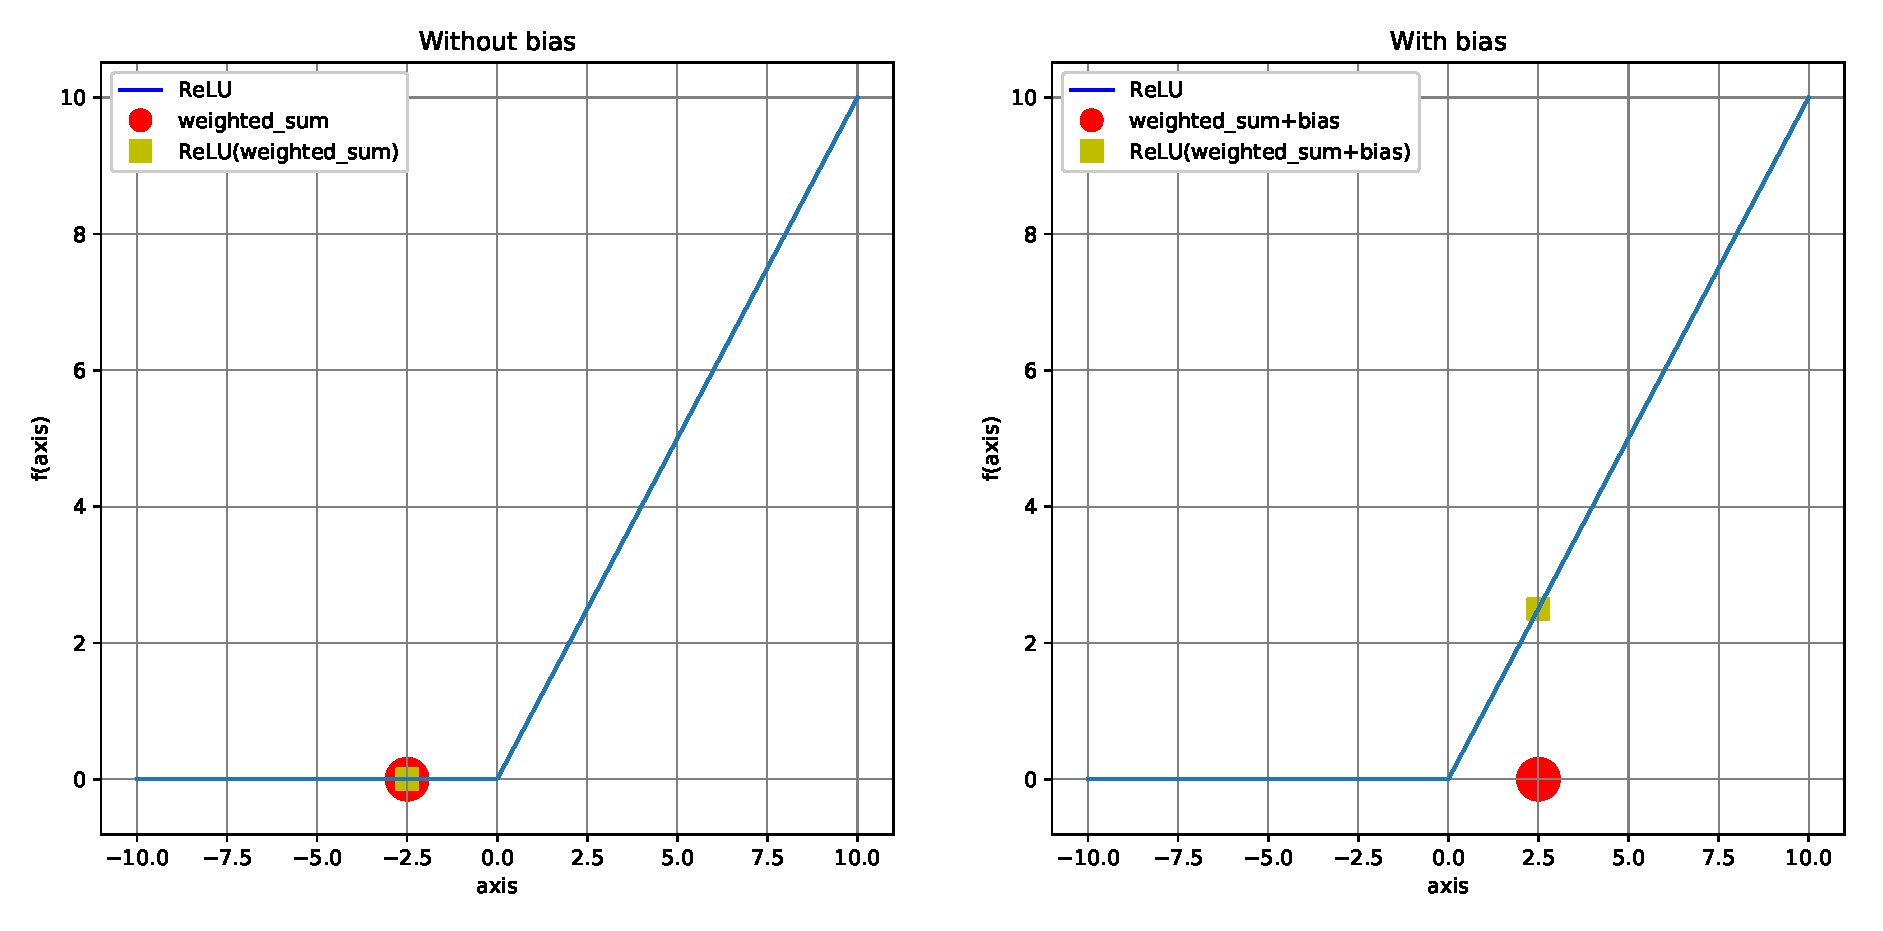
\includegraphics[width=0.95\textwidth]{Images/Plot/ReLU_bias.eps} 
\end{figure}
\end{frame}